\documentclass{beamer}
\usepackage{graphicx}
\usepackage{hyperref}
\usepackage{tikz}
\usetheme{Madrid}
\definecolor{ginger}{rgb}{0.69, 0.4, 0.0}
\usecolortheme{beaver}
\titlegraphic{
\includegraphics[width=2.5cm]{logo.png}
}
\title[Interaction of Laser Pulse With Plasma]{Interaction of Laser Pulse With Plasma}
\date{}
\institute[IIT Delhi]{\large Indian Institute of Technology, Delhi}
\author[]{Kulwinder Kaur (2021PHS7190)\\ Harikesh Kushwaha (2021PHS7181)\\[3mm]Adviser: Prof. Vikrant Saxena}
\vspace{0cm}
\begin{document}
{
\maketitle
\begin{frame}{Introduction}
    \frametitle{Introduction}
    \small
    Interaction of high intensity laser pulse with plasma gives rise to many interesting phenomena, one of which is high harmonic generation where high harmonics of the incident laser frequency is obtained after interaction with plasma. To understand the mechanism of high harmonic generation, we have to first understand the interaction of laser with plasma.\\
    \begin{itemize}
        \item Plasma is a quasineutral gas of charged and nuetral particles which exhibits collective behaviour.
        \item If an electron in plasma is displaced from its equilibrium position, it will start oscillating around its equilibrium position. The frequency of oscillation is given by\cite{chen} $\omega_p = \sqrt{\frac{n_pe^2}{m_e\epsilon_0}}$
        \item A plasma is called underdense if $\omega_p < \omega_l$ and overdense if $\omega_p > \omega_l$.
        \item The density at which $\omega_p = \omega_l$ is called critical density. We have $n_c = \frac{\omega_p^2m_e\epsilon_0}{e^2}$
        \item The simulation uses \textit{EPOCH}\cite{epoch}, a parallelised and fully relativistic implementation of particle in cell
              (PIC) algorithm.
    \end{itemize}
\end{frame}

\begin{frame}
    \small
    \frametitle{PIC Algorithm}
    PIC is a numerical approach that simulates a collection of particles that interact via external and self-induced electromagnetic fields.\cite{suciu}
    \begin{figure}
        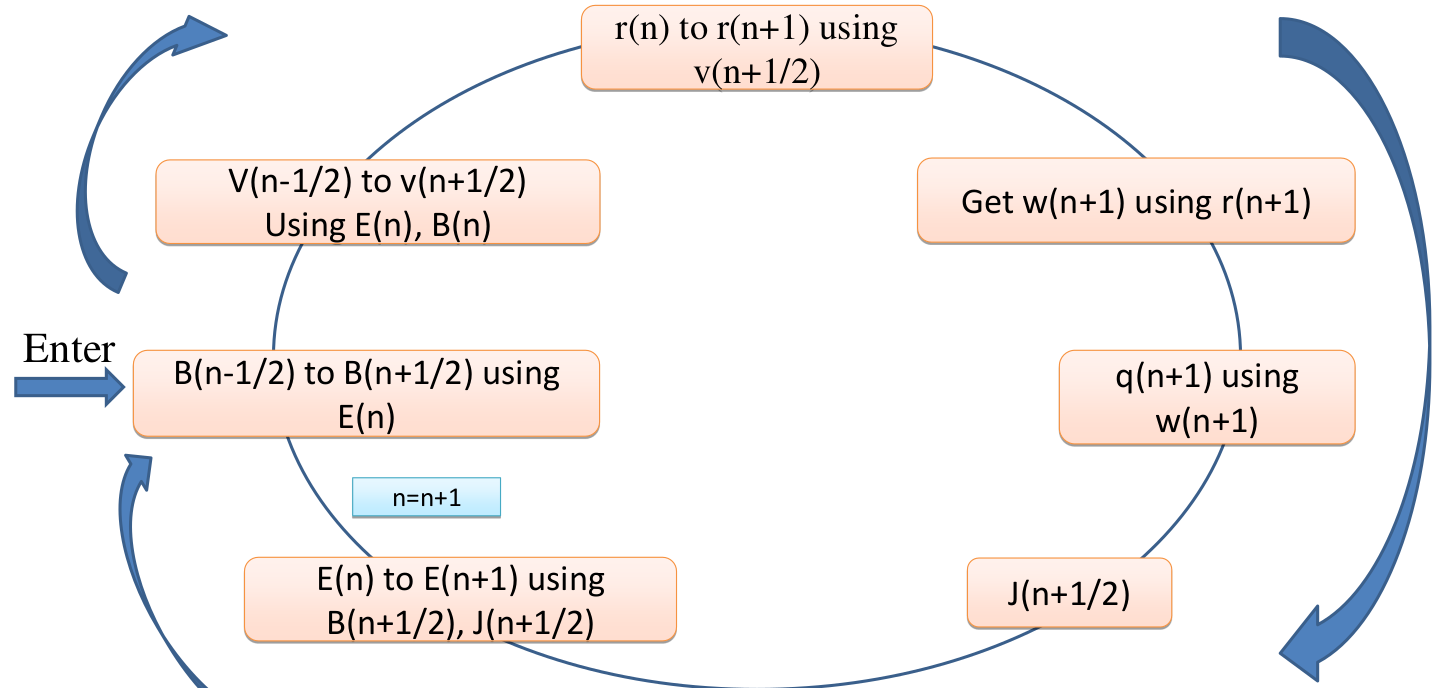
\includegraphics[width=10cm, height=6cm]{PIC.png}
        \centering
        \caption{The PIC Cycle}
    \end{figure}

\end{frame}
\begin{frame}
    \small
    \frametitle{Simulation Parameters}
    Normalize vector potential is defined as
    $
        a_0 = \frac{eE_0}{m w_l c}
    $
    . A laser is called relativistic if $a_0 \ge 1$.
    \begin{itemize}
        \item The simulation box extends for $20 \lambda _l$ and has total 1000 cells.
        \item  The plasma is placed at $x=0$ and with a thickess of $2\lambda_l$.  Number of macro particles per cell are 100.
        \item The plasma density $n_p$ is defined in terms of the critical density $n_c$ and is varied from 0.1 to 10. The vector potential $a_0$ is used as 0.1, 1.0 and 10.0.
    \end{itemize}

    \small
    \begin{columns}
        \begin{column}{0.5\textwidth}
            The envelope of the incident laser field varies according to\cite{lichters}
            \begin{equation*}
                P(t)=
                \begin{cases}
                     & \sin^2(\pi t/T) \text{ for } 0 \leq t \le T \\
                     & 0         \;      \text{ otherwise }
                \end{cases}
            \end{equation*}
            Where T is the pulse duration here taken as $T=10\tau$ with $\tau = 2\pi/\omega_l$ is the time of one laser cycle. The simulation is performed for $t=20\tau$.
        \end{column}
        \begin{column}{0.5\textwidth}  %%<--- here
            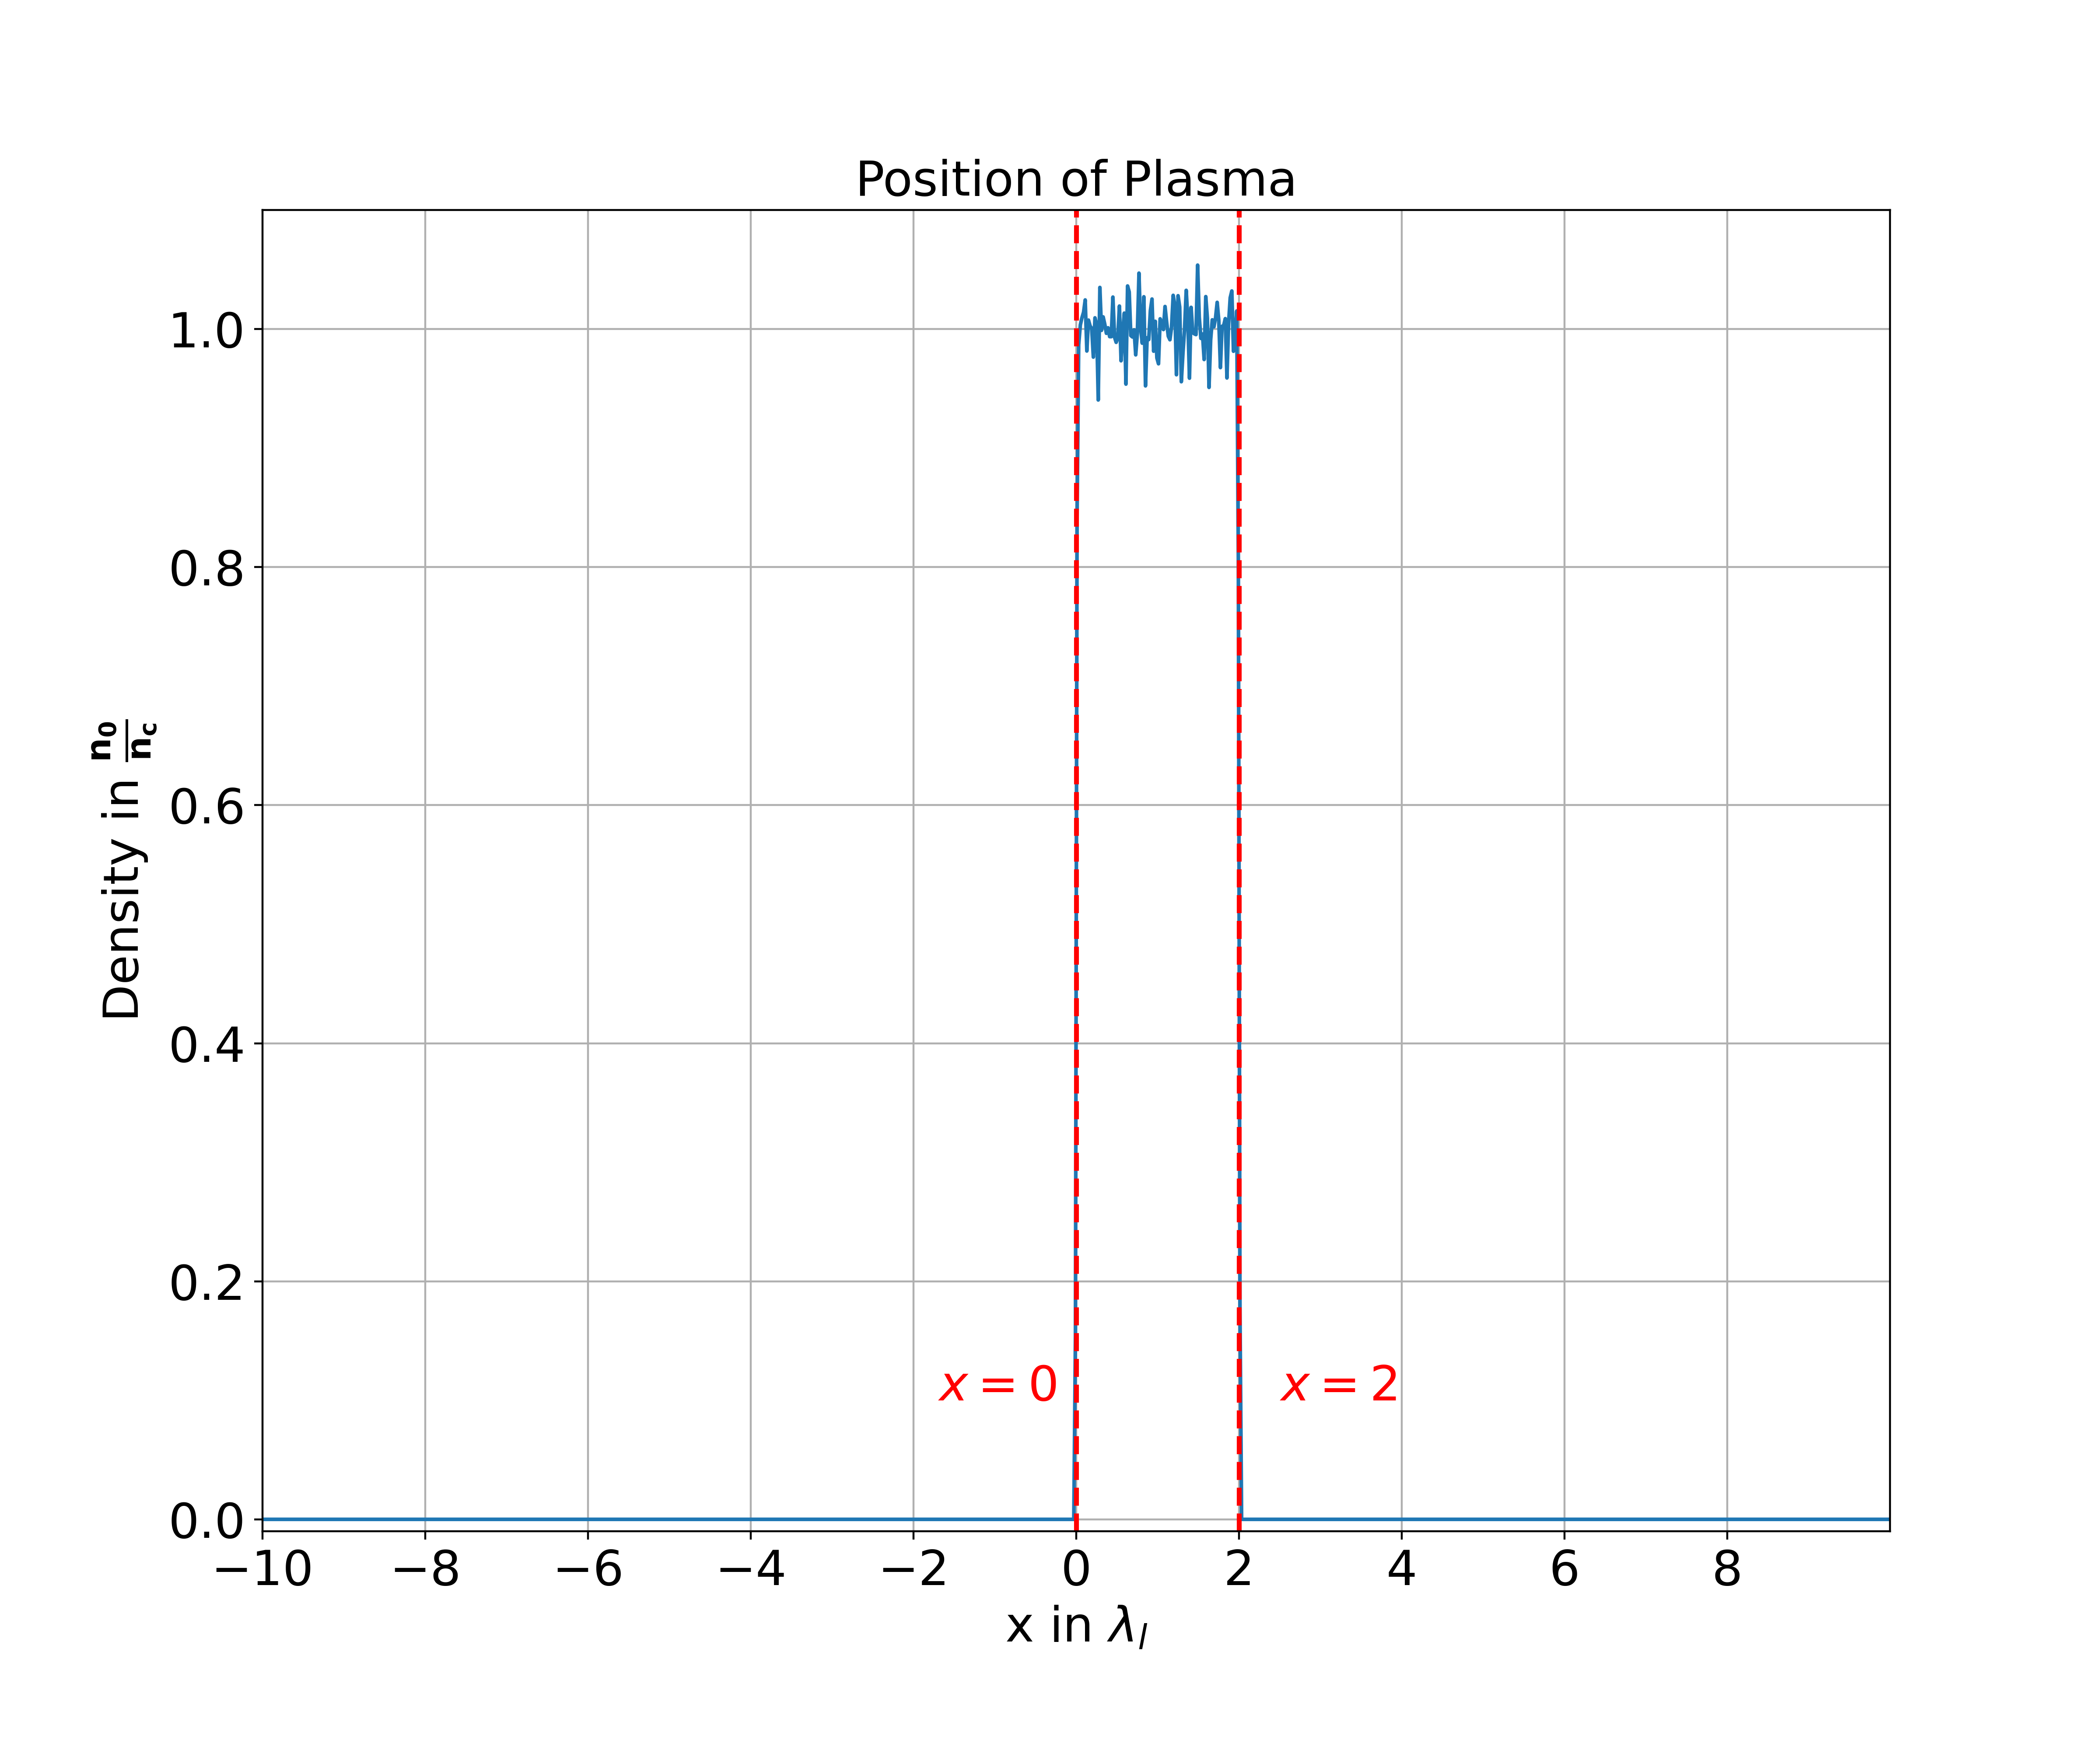
\includegraphics[width=6.5cm, height=4.5cm]{plasma.png}
        \end{column}
    \end{columns}
\end{frame}
\begin{frame}
    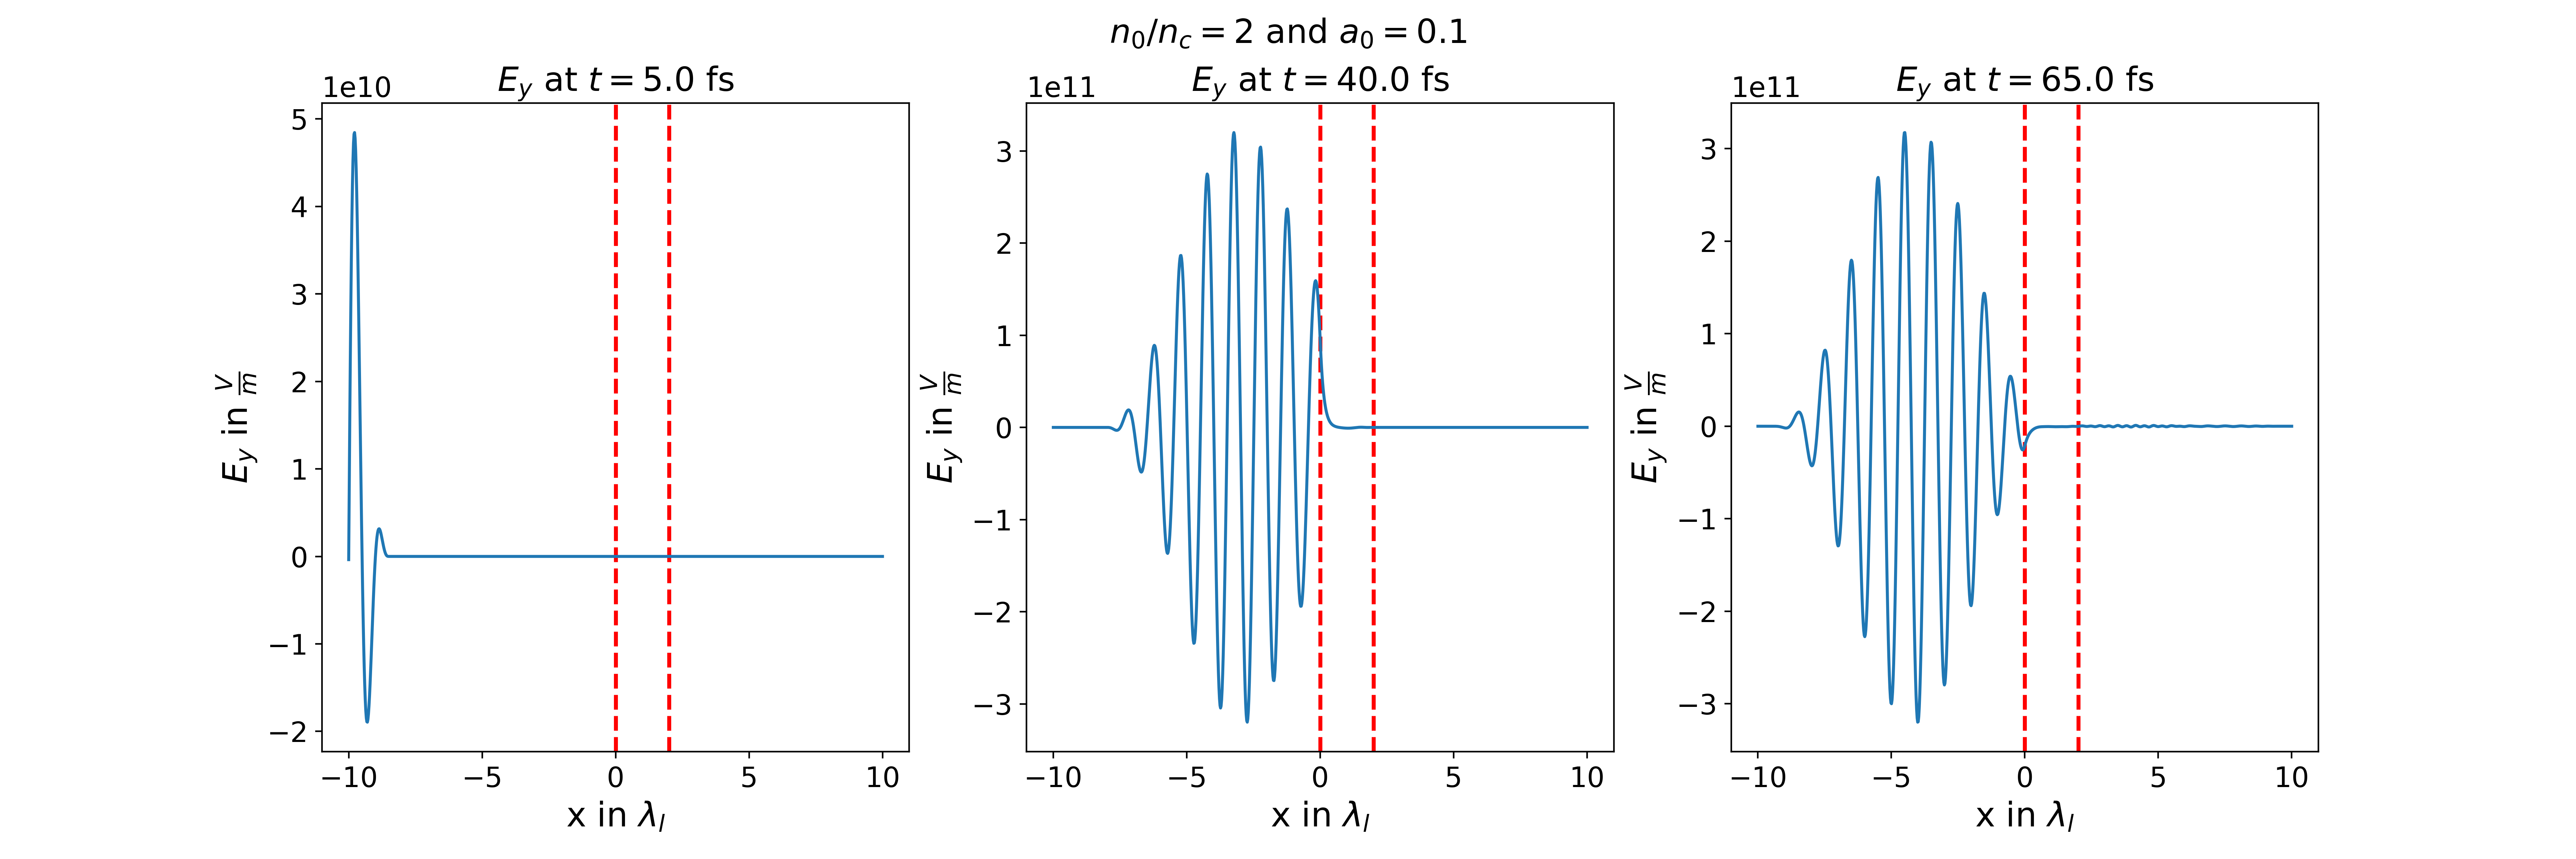
\includegraphics[width=12cm, height=3cm]{p1.png}
    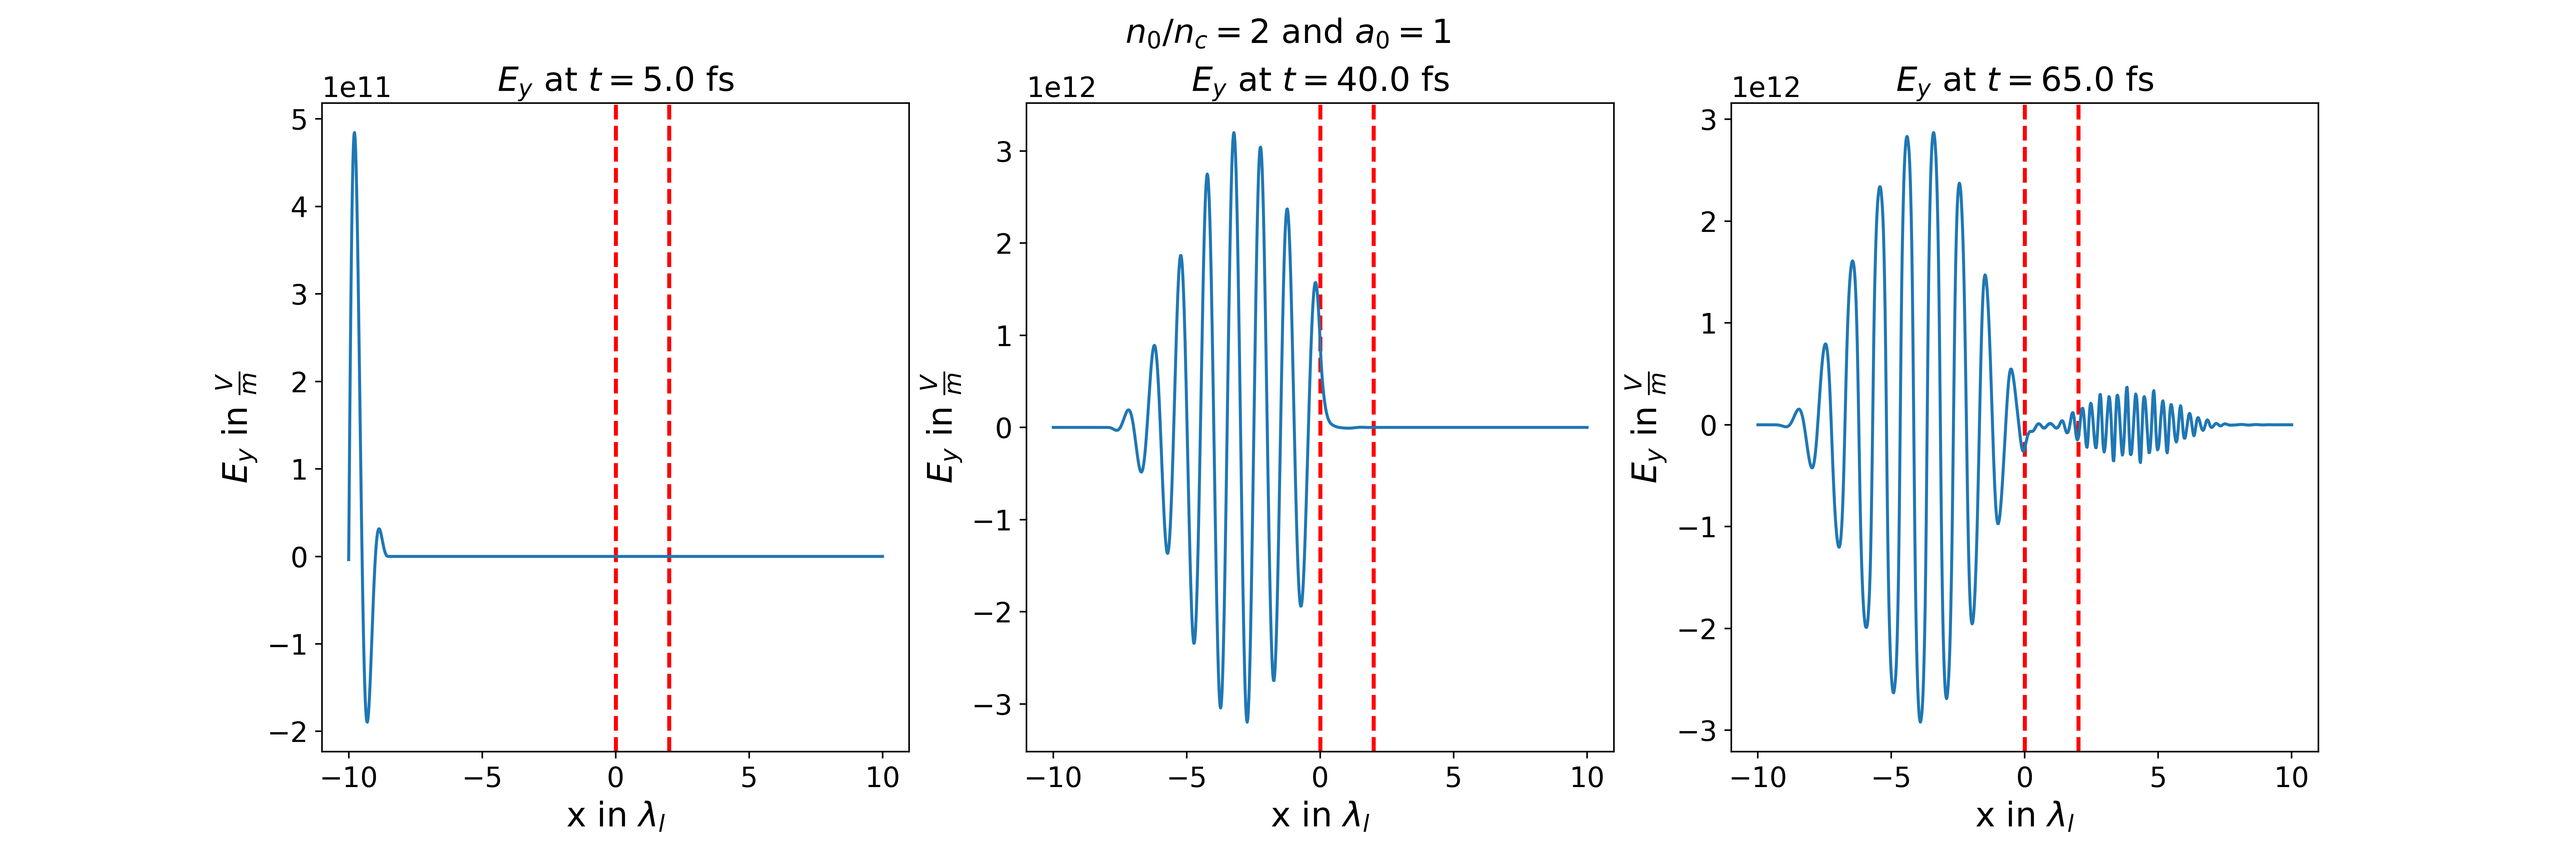
\includegraphics[width=12cm, height=3cm]{p2.png}
    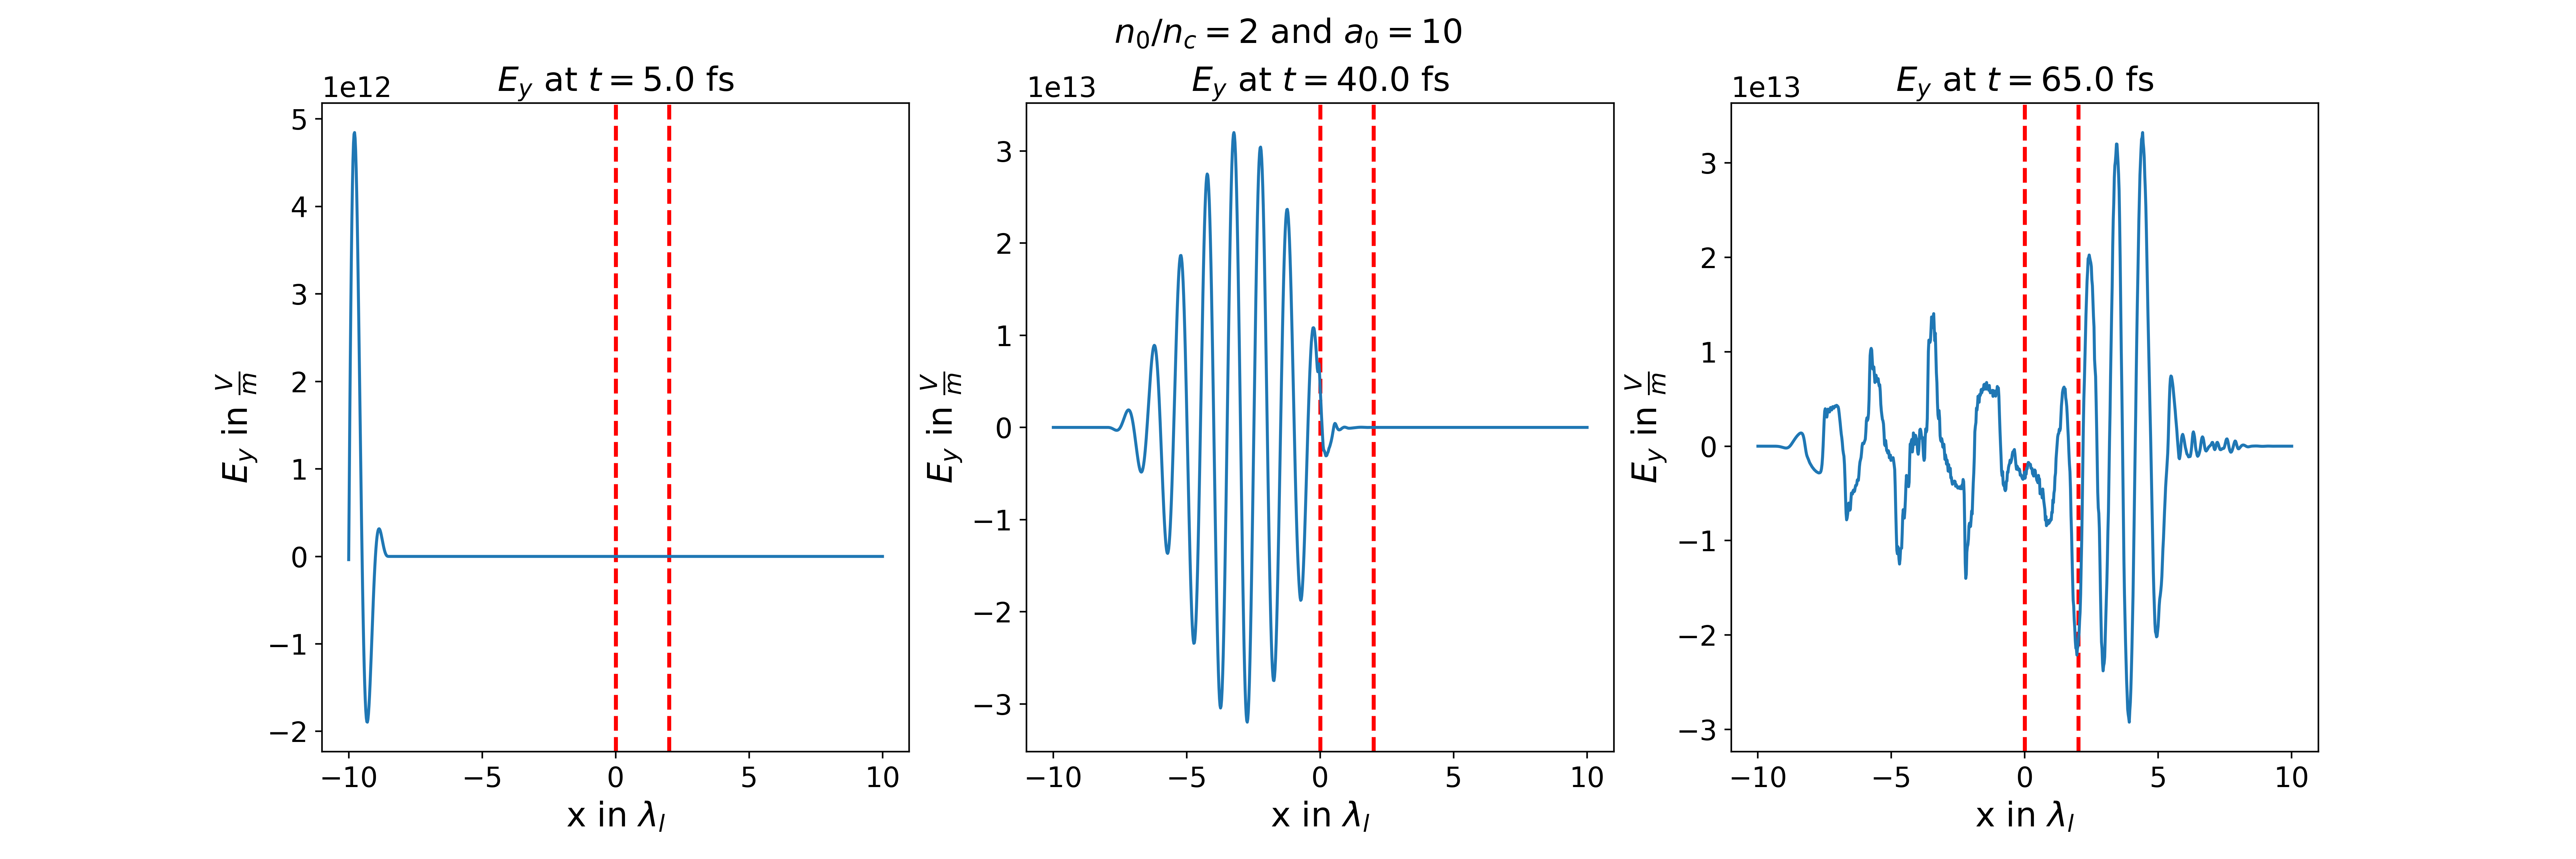
\includegraphics[width=12cm, height=3cm]{p3.png}
\end{frame}
\begin{frame}
    \frametitle{Result and Discussion}
    \small
    \begin{columns}
        \begin{column}{0.3\textwidth}
            We define a term
            $
                R= \frac{{E_{300}^2}-{E_{600}^2}}{{E_{300}^2}}
            $\\
            The plot of R with different ratio of $n_c$ and $n_0$ is shown in the figure 1 for different values of vector potential $a_0$. We find a shifting of the critical density for relativistic laser pulse.
        \end{column}
        \begin{column}{0.7\textwidth}
            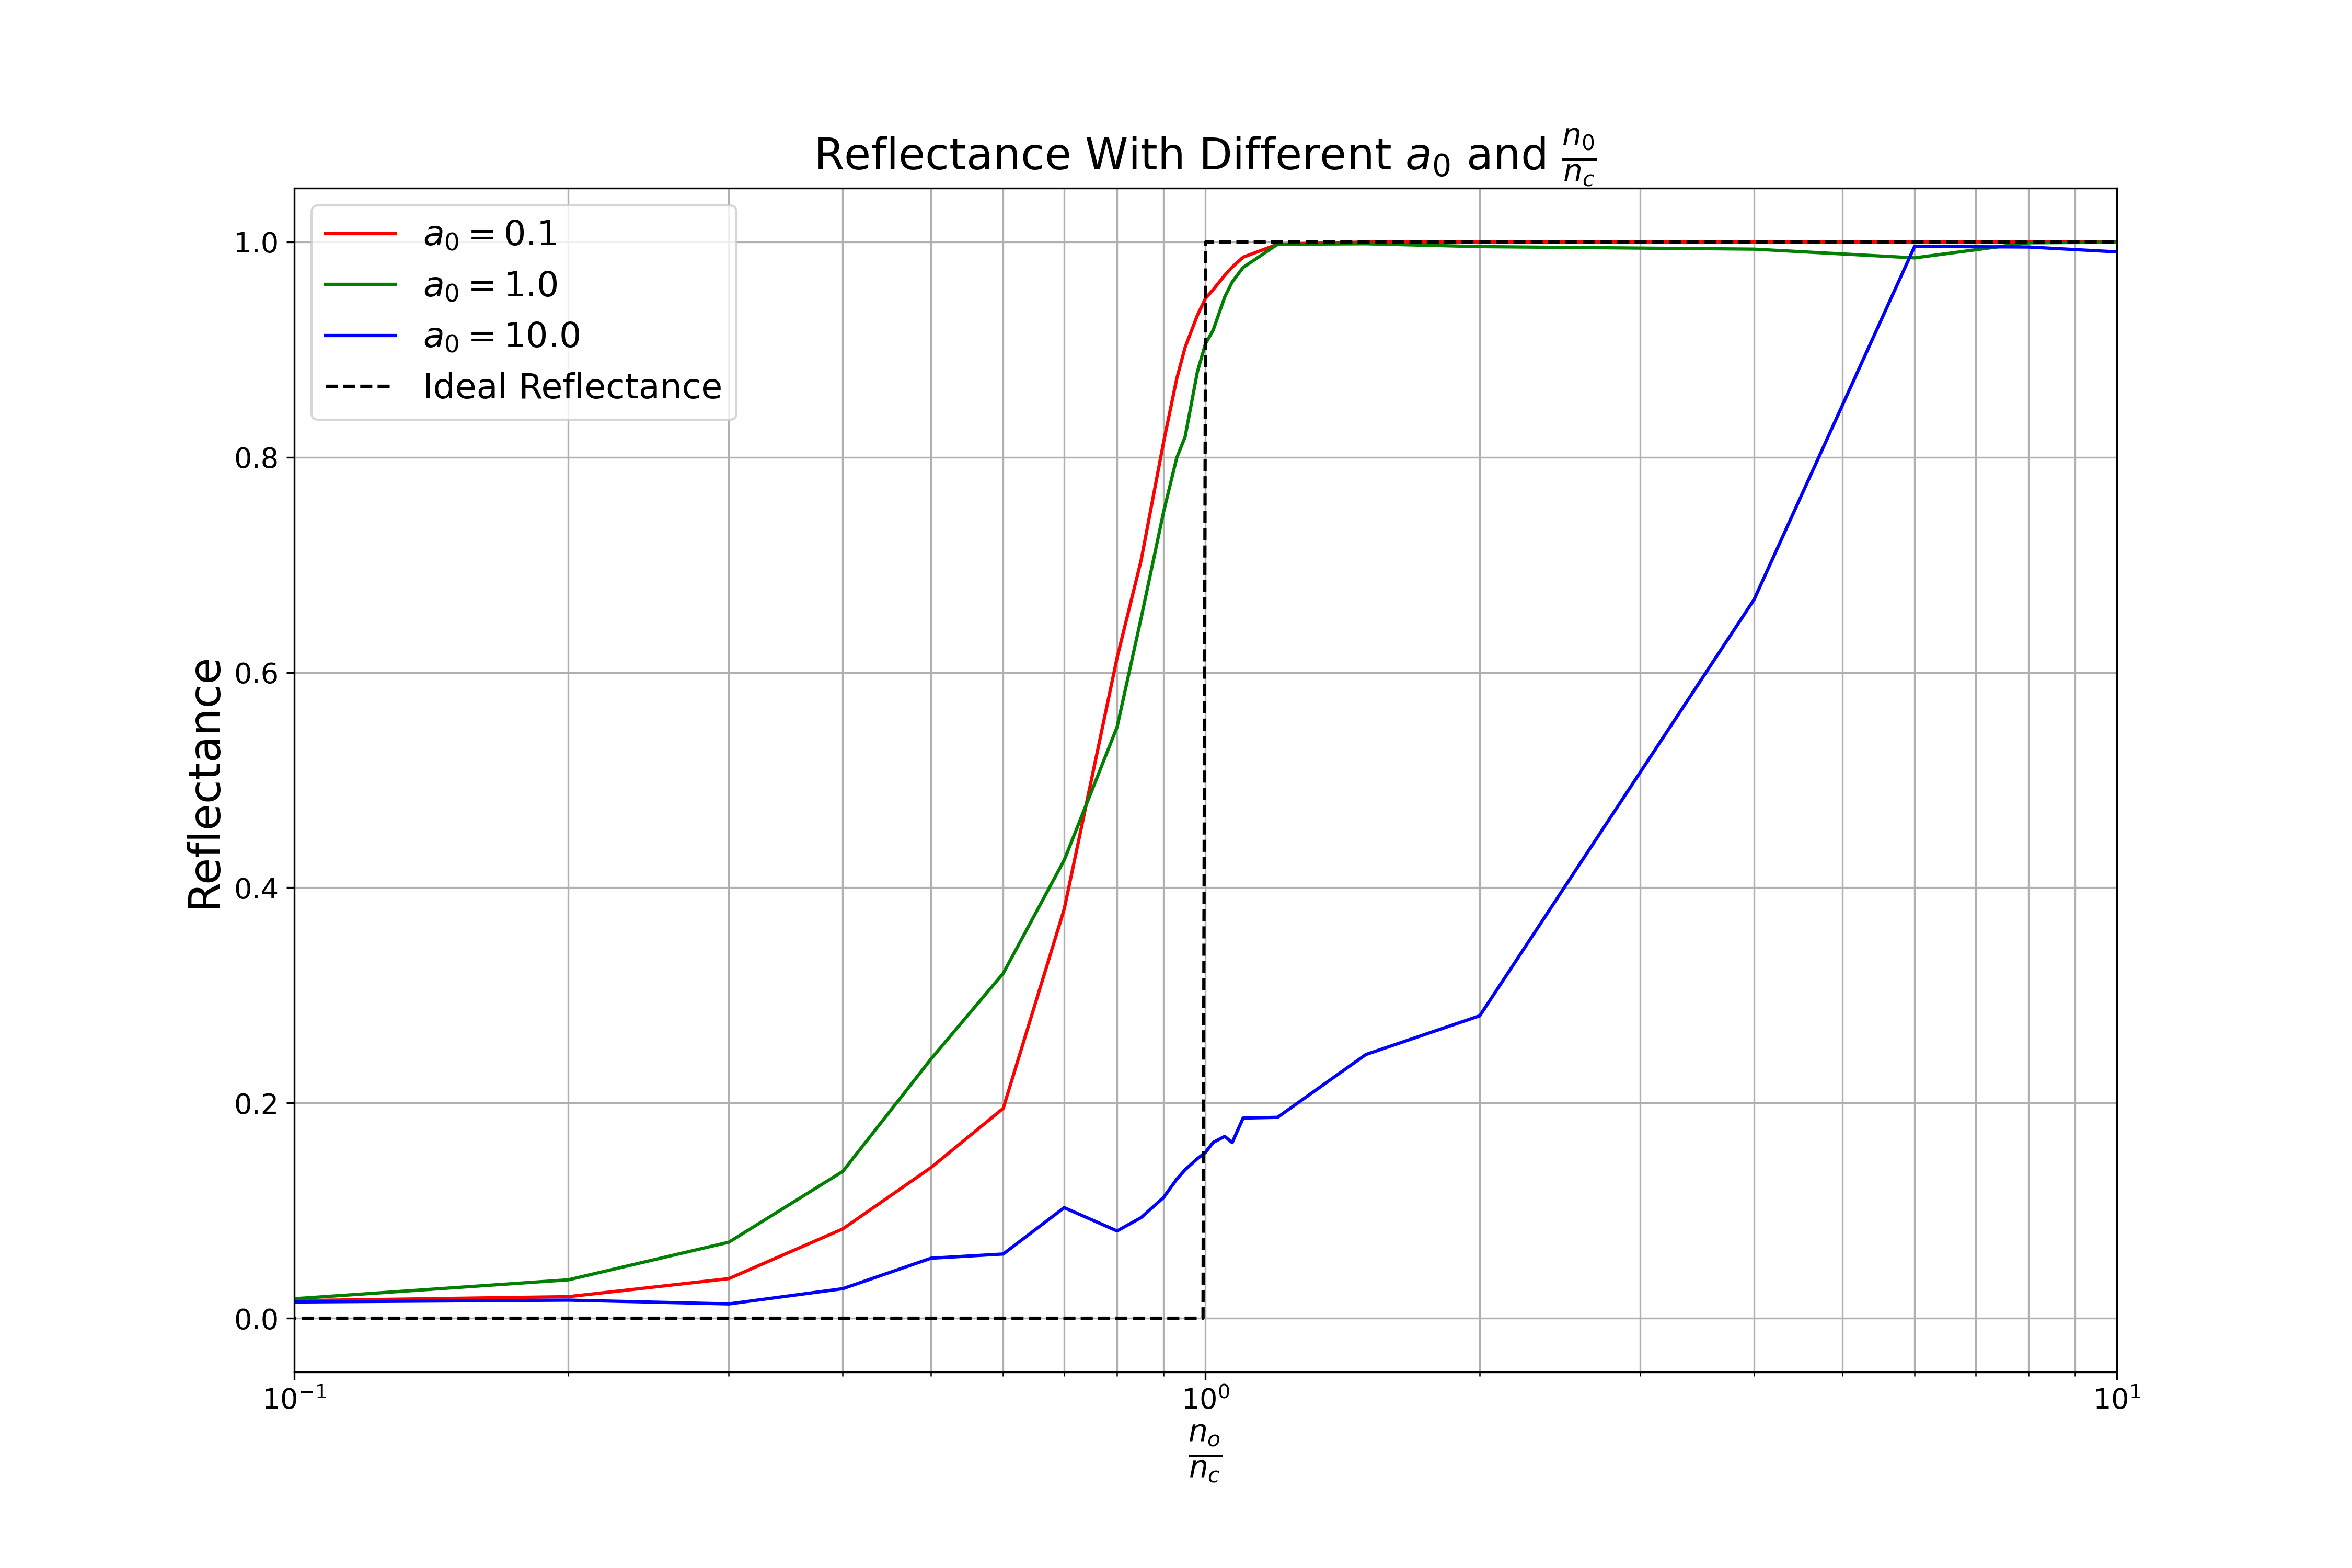
\includegraphics[width=8cm, height=6cm]{reflection.png}
        \end{column}
    \end{columns}
\end{frame}
\begin{frame}
    \small
    \begin{columns}
        \begin{column}{0.3\textwidth}
            The electron density with time is plotted for different $a_0$. The plot shows that the oscillation of electrons increases with increasing vector potential.
        \end{column}
        \begin{column}{0.7\textwidth}
            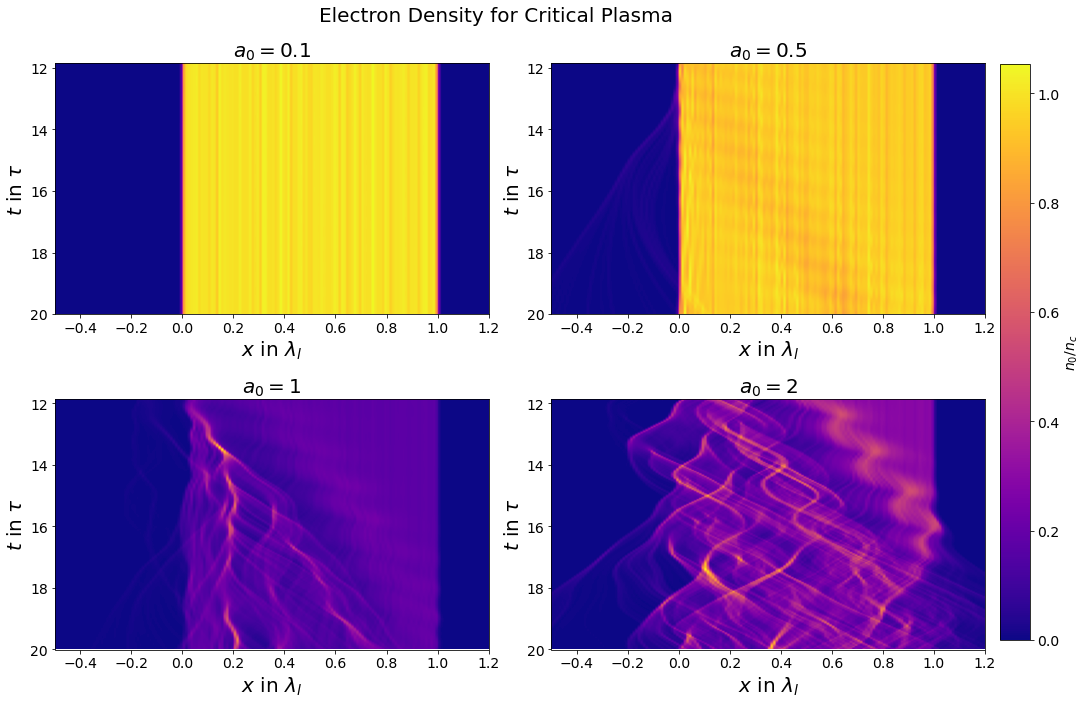
\includegraphics[width=8cm, height=6cm]{density.png}
        \end{column}
    \end{columns}
\end{frame}
\begin{frame}
    \frametitle{Conclusion and Future Plan of Work}
    \small
    \begin{itemize}
        \item A laser with extreme intensity drives relativistic oscillations of plasma particles. This results in shifting of effective plasma frequency because of the particles gaining mass.
        \item An overdense plasma reflects the laser back, forming a plasma mirror (PM). Now, if we let the surface of the PM oscillate, high harmonics of the incident laser pulse will be generated by Doppler effect.\cite{lichters} Future plan of work is to study these high harmonics.
    \end{itemize}
    \Large References
    \small
    \begin{thebibliography}{9}
        \bibitem{chen}
        Francis F. Chen
        Introduction to Plasma Physics and Controlled Fusion $3^{rd}$ Ed.

        \bibitem{epoch}
        Arber, T D Et al. Plasma Physics and Controlled Fusion 57 1-26 (2015)

        \bibitem{lichters}
        R. Lichters Et al. Physics of Plasmas 3, pp. 3425-3437 (1996)

        \bibitem{suciu}
        Alin Suciu Et al. 2020 15th Conference on Computer Science and Information Systems (FedCSIS), pp.381-385, 2020

    \end{thebibliography}
\end{frame}
\end{document}